\documentclass[fr]{../../../../../../eplexam}
\usepackage{../../../../../../eplunits}
\usepackage{circuitikz}
\usepackage{pgfplots}
\usepackage{enumitem}
\pgfplotsset{compat=newest}
\tikzset{meter/.style={draw,thick,circle,fill=white,minimum size =0.75cm,inner sep=0pt}}

\hypertitle{circmes-ELEC1370}{4}{ELEC}{1370}{2014}{Août}{All}
{Nicolas Verbeek\and Adrien Couplet\and Martin Van Essche\and Guillaume Gilson\and Guillaume Colinet}
{Claude Oestges, Bruno Dehez and Christophe Craeye}

\section{Question Oestges : phaseurs}
On considère le circuit suivant
\begin{center}
    \begin{circuitikz} 
    	\draw
		to[european resistor,l=$jX$, -*] (0,2.5) 
  		(2.5,2.5) to[american current source,l=$2\angle\ang{0}$A] (0,2.5)
  		(2.5,2.5) to [american voltage source,l=$12\angle\ang{0}$V] (5,2.5)
  		(2.5,0) to[L,l_=j$\SI{4}{\ohm}$,-*] (2.5,2.5)
 		(5,2.5) to[R,v=$V_o$,l=$\SI{2}{\ohm}$,*-] (5,0)
 		(0,0) -- (5,0)
 		(0,2.5) -- (0,4) to[R,l=$R$] (5,4) -- (5,2.5);
 	\end{circuitikz}
\end{center}
On mesure une tension $V_o=5.5\angle\ang{-101.1}$V. On demande de calculer
\begin{enumerate}
    \item Les valeurs de $R$ et de $X$ (ces valeurs sont réelles)
    \item la tension (amplitude et phase) aux bornes de la source de courant de 2A, ainsi que sa valeur efficace.
    \item la puissance délivrée par la source de tension
\end{enumerate}

\begin{solution}
Solutions finales (contrôlées avec LTSpice):
\begin{enumerate}
    \item $R=\SI{11.38}{\ohm}$ et $X=\SI{0.562}{\ohm}$.
    \item $V_s = 14.85\angle\ang{25.74}$ V et $I_s = 3.33 \angle\ang{-101.27}$ A
    \item $P=\SI{-3.9}{\watt}$
\end{enumerate}
\end{solution}

\section{Question Oestges : Bode et quadripôles}
On considère le circuit de filtrage suivant
\begin{center}\centering
	\begin{circuitikz}
		\draw
		(0,1) node [above]{$V_\text{in}$} to [short,o-] (1,1) 
		to [R, l=$R_1$] (2,1)
		(6,0.5) node[op amp] (opamp) {}
		(opamp.-) to [C,l_=$C_1$] (2,1) 
		(opamp.+) to [short] (4,0)
		(opamp.out) to [short] (8,0.5)
		(4.5,1) to [short,*-*] (4.5,2.5) to [R,l=$R_2$,-*] (8,2.5) -- (8,0.5)
		(4.5,2.5) -- (4.5,4) to [C,l=$C_2$] (8,4) -- (8,2.5)
		(4,0) -- (4,-0.5) node [ground] {}
		(8,0.5) to [short,*-o] (9,0.5) node [above]{$V_\text{out}$};
	\end{circuitikz}
\end{center}
où l'amplificateur opérationnel est considéré comme idéal et $C_1 = C_2 = \SI{10}{\nano\farad}$, $R_1 = \SI{5}{\kilo\ohm}$ et $R_2 = \SI{1}{\kilo\ohm}$. On demande de
\begin{enumerate}
    \item Déterminer l'expression analytique (sans remplacer par les valeurs) de la matrice \textbf{G} du quadripôle ainsi formé.
    \item Tracer le diagramme de Bode (amplitude et phase) du gain $g_f$ (pour les valeurs données des éléments). Quelle est la fonction de ce circuit (passe-haut, passe-bas, passe-bande) ? Quelle est la bande passante du filtre ?
    \item Si la charge est une impédance de $\SI{1}{\kilo\ohm}$, déterminer la valeur de l’impédance d’entrée $Z_\text{in}$, respectivement à 1, 10 et $\SI{100}{\kilo\hertz}$.
\end{enumerate}

\begin{solution}
\begin{enumerate}
    \item La matrice \textbf{G} du quadripôle
    \[ G = 
    \begin{pmatrix}
    g_i & g_r\\
    g_f & g_o
    \end{pmatrix}
     = \begin{pmatrix}
    \frac{j\omega C_1}{1+j\omega R_1 C_1} & 0\\
    \frac{-j \omega R_2 C_1}{(1+j \omega C_2 R_2)(1+j \omega C_1 R_1)} & 0
    \end{pmatrix} \]
    \item Pour les valeurs données, nous avons $g_f = \frac{-j \omega 10^{-5}}{(1+5j \omega 10^{-5})(1+j \omega 10^{-5})} $
    Il s'agit d'un filtre passe bande.
    \item Via le tableau des caractéristiques externes, on trouve
    \[ Z_\text{in} = \frac{1}{g_i} = \frac{1+j\omega R_1 C_1}{j\omega C_1} \]
\end{enumerate}
\end{solution}

\section{Question Dehez : circuit magnétiques couplés}
On considère le circuit suivant 
\begin{center}
    \begin{circuitikz}
        \draw (0,0) to[R,l=\SI{12}{\ohm},*-] ++(-2,0) to[american voltage source,l=$12\angle\ang{0}\,\si{\volt}$] ++(0,2) to[R,l=\SI{2}{\ohm}] ++(2,0) to[R,l=\SI{4}{\ohm}] ++(0,-2);
        \draw (0,0) to[R,l=\SI{4}{\ohm},-*] ++(0,-2) to[short] ++(-2,0) to[american voltage source,l=$24\angle\ang{0}\,\si{\volt}$,-*] ++(0,2);
        \draw (0,0) to[C,l=\SI{-j2}{\ohm}] ++(3,0) coordinate (b1) to[L,l_=\SI{j4}{\ohm}] ++(0,-2) to[short] ++(-3,0);
        \draw (b1) node[below left]{$\bullet$};
        \draw ($ (b1) + (1,-2) $) coordinate (b4) to[L,l_=\SI{j3}{\ohm}] ++(0,2) coordinate (b2) to[C,l=\SI{-j1}{\ohm},-*] ++(3,0) to[short, -o] ++(1,0) coordinate (v1) node[right]{$+$};
        \draw (b4) to[short,-*] ++(3,0) coordinate (c) to[R,l=\SI{2}{\ohm}] ++(0,2);
        \draw (c) to[short,-o] ++(1,0) coordinate (v2) node[right]{$-$};
        \draw (b4) node[above right]{$\bullet$};
        
        \draw [<->,>=stealth] ($ (b1) + (-0.2,0.2) $)  to [bend left] node[pos=0.5,above] {\SI{-j1}{\ohm}} ($ (b2) + (0.2,0.2) $);
        \draw [<-,>=stealth] ($ (v1) + (0,-0.2) $)  to [bend left] node[pos=0.5,right] {$V_o$} ($ (v2) + (0,0.2) $);
    \end{circuitikz}
\end{center}
\begin{enumerate}
    \item Calculer le facteur de dispersion entre les deux inductances couplées magnétiquement.
    \item Calculer l'amplitude et la phase de la tension $V_o$.
\end{enumerate}
On souhaite mesurer l’amplitude de cette tension au moyen d’un voltmètre idéal, mais dont le fond d’échelle, de \SI{100}{\milli\volt}, n’est à priori pas adapté. L’usage d’un transformateur (supposé idéal) est alors envisagé pour adapter la tension mesurée par l’ampèremètre.
\begin{center}
    \begin{circuitikz}
        \draw (0,0) to[R,l=\SI{12}{\ohm},*-] ++(-2,0) to[american voltage source,l=$12\angle\ang{0}\,\si{\volt}$] ++(0,2) to[R,l=\SI{2}{\ohm}] ++(2,0) to[R,l=\SI{4}{\ohm}] ++(0,-2);
        \draw (0,0) to[R,l=\SI{4}{\ohm},-*] ++(0,-2) to[short] ++(-2,0) to[american voltage source,l=$24\angle\ang{0}\,\si{\volt}$,-*] ++(0,2);
        \draw (0,0) to[C,l=\SI{-j2}{\ohm}] ++(3,0) coordinate (b1) to[L,l_=\SI{j4}{\ohm}] ++(0,-2) to[short] ++(-3,0);
        \draw (b1) node[below left]{$\bullet$};
        \draw ($ (b1) + (1,-2) $) coordinate (b4) to[L,l_=\SI{j3}{\ohm}] ++(0,2) coordinate (b2) to[C,l=\SI{-j1}{\ohm},-*] ++(3,0) to[short, -o] ++(1,0) coordinate (v1);
        \draw (b4) to[short,-*] ++(3,0) coordinate (c) to[R,l=\SI{2}{\ohm}] ++(0,2);
        \draw (c) to[short,-o] ++(1,0) coordinate (v2);
        \draw (b4) node[above right]{$\bullet$};
        
        \draw [<->,>=stealth] ($ (b1) + (-0.2,0.2) $)  to [bend left] node[pos=0.5,above] {\SI{-j1}{\ohm}} ($ (b2) + (0.2,0.2) $);
        \draw [<-,>=stealth] ($ (v1) + (0,-0.2) $)  to[] node[pos=0.5,right] {$V_o$} ($ (v2) + (0,0.2) $);
        
        \draw (v1) to[short,o-] ++(1,0) coordinate (t1) to[L] ++(0,-2) coordinate (t3) to[short,-o] ++(-1,0);
        \draw ($ (t1) + (1,-2) $)    coordinate (t4) to[L] ++(0, 2) coordinate (t2) to[short] ++(1,0) to[short] ++(0,-1) node[meter]{\small V} to[short] ++(0,-1) to[short] ++(-1,0);
        
        \draw (t2) node[below right]{$\bullet$};
        \draw (t1) node[below left]{$\bullet$};
        \draw[thick] ($ (t1) + (0.4,-0.2) $)  -- ($ (t3) + (0.4,0.2) $);
        \draw[thick] ($ (t2) + (-0.4,-0.2) $) -- ($ (t4) + (-0.4,0.2) $);
        
        \draw[white] ($ (t1) + (-0.2,0.2) $)  to[] node[black,pos=0.5,above] {$n:1$} ($ (t2) + (0.2,0.2) $);
    \end{circuitikz}
\end{center}
\begin{enumerate}[resume]
    \item Calculer la valeur idéale que devrait prendre le rapport de transformation $n$ de ce transformateur pour avoir une mesure correspondant au fond d’échelle du voltmètre.
\end{enumerate}

\begin{solution}
	\begin{enumerate}
    \item Le coefficient de dispersion $\sigma$ est définit comme 
        \[ \sigma = 1 - \frac{M^2}{L_1L_2} = 1 - \frac{1}{12} = \frac{11}{12} \]
    \item
    \begin{center}
            \begin{circuitikz}
                \draw (0,0) to[R,i>_=$I_2$,l=\SI{12}{\ohm},*-] ++(-2,0) to[american voltage         source,l=$12\angle\ang{0}\,\si{\volt}$] ++(0,2) to[R,l=\SI{2}{\ohm},i=$I_1$] ++(2,0) to[R,l=\SI{4}{\ohm}] ++(0,-2);
                \draw (0,0) to[R,l=\SI{4}{\ohm},-*] ++(0,-2) to[short] ++(-2,0) to[american voltage source,l=$24\angle\ang{0}\,\si{\volt}$,-*] ++(0,2);
                \draw (0,0) to[C,l=\SI{-j2}{\ohm},i=$I_3$] ++(3,0) coordinate (b1) to[L,l_=\SI{j4}{\ohm}] ++(0,-2) to[short] ++(-3,0);
                \draw (b1) node[below left]{$\bullet$};
                \draw ($ (b1) + (1,-2) $) coordinate (b4) to[L,l_=\SI{j3}{\ohm}] ++(0,2) coordinate (b2) to[C,l=\SI{-j1}{\ohm},i<_=$I_4$,-*] ++(3,0) to[short, -o] ++(1,0) coordinate (v1) node[right]{$+$};
                \draw (b4) to[short,-*] ++(3,0) coordinate (c) to[R,l=\SI{2}{\ohm}] ++(0,2);
                \draw (c) to[short,-o] ++(1,0) coordinate (v2) node[right]{$-$};
                \draw (b4) node[above right]{$\bullet$};
        
                \draw [<->,>=stealth] ($ (b1) + (-0.2,0.2) $)  to [bend left] node[pos=0.5,above] {\SI{-j1}{\ohm}} ($ (b2) + (0.2,0.2) $);
                \draw [<-,>=stealth] ($ (v1) + (0,-0.2) $)  to [bend left] node[pos=0.5,right] {$V_o$} ($ (v2) + (0,0.2) $);
                
                \draw (-1,1) node[scale=2]{$\circlearrowright$};
                \draw (-1,-1) node[scale=2]{$\circlearrowright$};
                \draw (1.5,-1) node[scale=2]{$\circlearrowright$};
                \draw (5.5,-1) node[scale=2]{$\circlearrowright$};
                
            \end{circuitikz}
        \end{center}
        En effectuant quatre fois la loi des mailles, on obtient le système suivant:
        \[  \begin{cases}
            12 - 6I_1 - 12I_2 = 0 \\
            24 + 12I_2 - 4(I_1-I_2-I_3) = 0 \\
            4(I_1-I_2-I_3) + 2j I_3 - 4j I_3 - j I_4 = 0 \\
            3j I_4 + j I_3 - j I_4 + 2I_4 = 0
            \end{cases} \]
        Soit encore, en réécrivant ce système sous forme matricielle:
        \[  \begin{bmatrix}
            6 & 12 & 0 & 0 \\
            4 & -16 & -4 & 0 \\
            4 & -4 & -4-2j & -j \\
            0 & 0 & j & 2+2j 
            \end{bmatrix} \begin{bmatrix}
            I_1 \\ I_2 \\ I_3 \\ I_4
            \end{bmatrix} = \begin{bmatrix} 
                12 \\ 24 \\ 0 \\ 0
            \end{bmatrix} \]
        D'où, en résolvant:
        \[  \begin{cases}
            I_1 &= 4.95\angle\ang{-13.43}\,\si{\ampere} \\
            I_2 &= 1.52\angle\ang{157.77}\,\si{\ampere} \\    
            I_3 &= 5.61\angle\ang{-37.88}\,\si{\ampere} \\ 
            I_4 &= 1.99\angle\ang{-172.87}\,\si{\ampere} 
            \end{cases} \]
        On peut alors déterminer la tension $V_o$:
        \[ V_o = -2I_4 = 3.97\angle\ang{7.13}\,\si{\ampere} \]
    \textbf{Note:} Une méthode équivalente (plus simple au niveau calculs) est de d'abord trouver le dipôle équivalent de Thévenin de la partie gauche du circuit (on trouve $V_\text{th} = 16$V et $Z_\text{th} = 2-2j$), et puis résoudre le système (réduit).
    \item On souhaite observer au voltmètre une tension ne dépassant pas les \SI{100}{\milli\volt}. Pour cela nous utiliserons la formule liant les tensions et les nombres de spires de part et d'autre d'un transformateur
        \[ \frac{V_1}{V_2} = \frac{N_1}{N_2} \Leftrightarrow \frac{V_o}{V_m} = n\]
        On pose la condition:
        \[ V_m < \SI{100}{\milli\volt} \Rightarrow \frac{V_o}{n} < \SI{100}{\milli\volt} \Rightarrow n > \frac{V_o}{0.1} = 39.7 \]
        On en conclut que pour avoir une mesure correspondant au fond d'échelle du voltmètre, il faut que le nombre de spire $n$ côté circuit vaille au minimum 40 spires. 
\end{enumerate}
\end{solution}

\section{Question Craeye : transitoire} 
Soit le circuit suivant dont l'interrupteur 2V s'ouvre et l'interrupteur 1V se ferme en $t=0$.
\begin{center}
    \begin{circuitikz} 
    	\draw
 		(0,0) -- (4,0)
 		(-1.5,0) -- (0,0)
 		(-1.5,0) to[american voltage source,l=1V] (-1.5,2.5) to [closing switch,l=$t{=}0$] (-1.5,5) -- (0,5)
 		(0,0) to[american voltage source,l=2V] (0,2.5) to [opening switch,l=$t{=}0$] (0,5) to [R,l=$R$,*-] (1.8,5)
 		(1.8,5) to [L,l=$L$] (4,5)
		(5,3.6) to [open, v^=$V_o$] (5,1)
		(4,5) to [C,l=$C$] (4,0);
	\end{circuitikz}
\end{center}
On demande la tension $V_o$ en $t>0$ avec les données numériques suivantes :
$R=\SI{2.5}{\kilo\ohm}$, $L=\SI{0.5}{\milli\henry}$, $C = \SI{0.5}{\nano\farad}$

\begin{solution}
L'expression analytique de la solution est
\[ V_o(t) = \left[1-\frac{1}{3} e^{-4\cdot10^6 t} + \frac{4}{3} e^{-10^6 t}\right]u(t) \]

Le graphe ressemble à
\begin{center}
    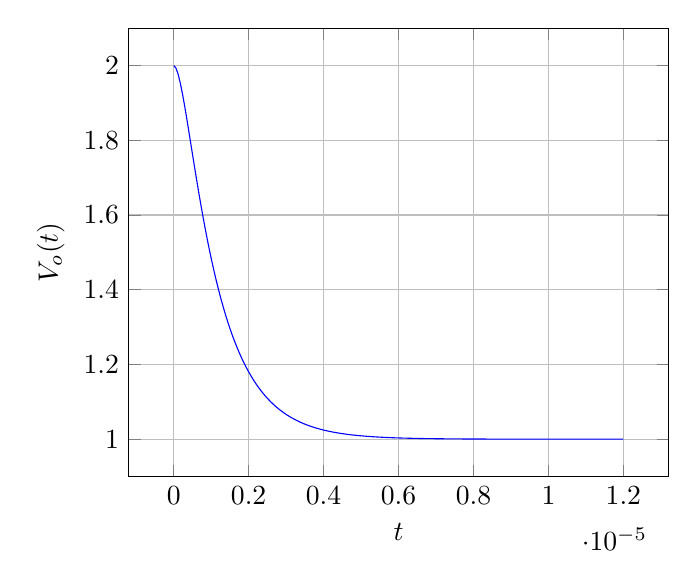
\begin{tikzpicture}
        \begin{axis}[enlargelimits=true,grid=major,ylabel=$V_o(t)$,xlabel=$t$]
            \addplot [blue,domain=0:0.000012,samples=200]{1-(1/3)*e^(-4*(10^6)*x)+(4/3)*e^(-10^6*x)};
        \end{axis}
    \end{tikzpicture}
\end{center}
\end{solution}

\end{document}
